\documentclass{beamer}
\usepackage{graphicx} % Omogoča vključitev slik
\setbeamertemplate{footline}[frame number]
\setbeamercolor{section in toc}{fg=black} 

% Naslov, avtor in datum
\title{Predstavitev 1.naloge v MATLAB-u}
\author{Aljaž Oskar Livk, 23221052}
\date{\today}

\begin{document}

% 1. Prosojnica: Uvodna prosojnica
\begin{frame}
    \titlepage % Uporabi naslov, avtorja in datum
\end{frame}

% 2. Prosojnica: Kazalo vsebine
\begin{frame}{Kazalo vsebine}
    \tableofcontents
\end{frame}

% 3. Prosojnica: Predstavitev vsebine datoteke in MATLAB funkcije
\section{1. Vsebina datoteke naloga1\_1.txt }
\begin{frame}{1. Vsebina datoteke naloga1\_1.txt}
    \begin{itemize}
        \item Prva vrstica: Ime podatkovne datoteke.
        \item Druga vrstica: Število vrstic in število podatkov v vsaki vrstici.
        \item Število podatkov: (vpišite število podatkov).
        \item Podatki predstavljajo (opis podatkov, npr. časovne točke in meritve).
    \end{itemize}
    
    \vspace{1em} % Dodamo nekaj prostora med elementi
    
    \textbf{1.1 MATLAB funkcija za branje datoteke:}
    \begin{itemize}
        \item Funkcija: \texttt{fscanf} (ali \texttt{fgetl}, \texttt{importdata} - glede na vašo izbiro).
        \item Vhodni podatki: Ime datoteke, format branja.
        \item Izhodna vrednost: Prebrane vrednosti, shranjene v spremenljivkah.
    \end{itemize}
\end{frame}

% 4. Prosojnica: Graf P(t)
\section{2. Graf P(t)}
\begin{frame}{2. Graf P(t)}
    \begin{itemize}
        \item Graf prikazuje odvisnost P od časa t.
    \end{itemize}
    
    \begin{figure}
        \centering
        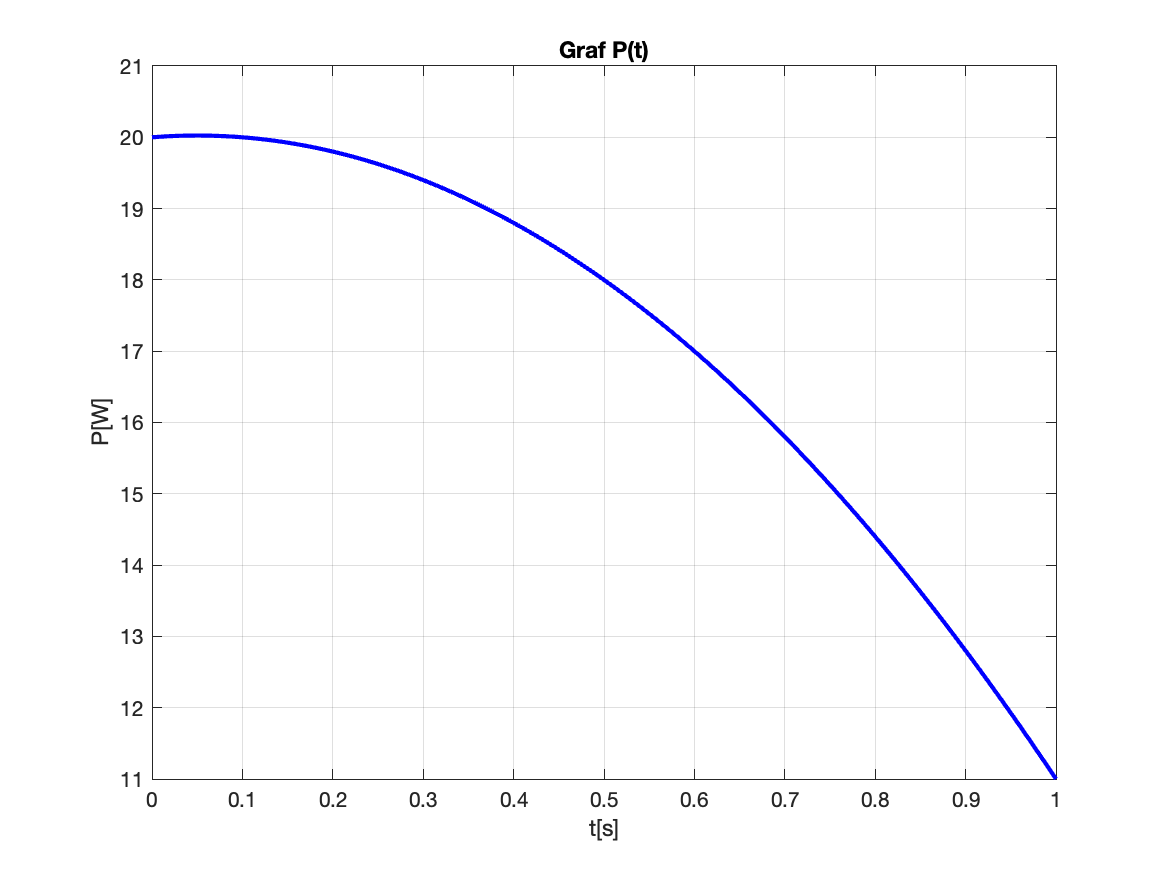
\includegraphics[width=0.8\textwidth]{Graf_P_t.png} % Shranite sliko grafa kot graf_P_t.png
        \caption{Graf P(t) izrisan v MATLAB-u}
    \end{figure}
\end{frame}

% 5. Prosojnica: Trapezna formula za integral in rešitev
\section{3. Trapezna formula za integral}
\begin{frame}{3. Trapezna formula za integral}
    \textbf{Trapezna formula za izračun integrala:}
    
    \[
    \int_a^b f(x) \, dx \approx \frac{b - a}{2} \sum_{i=1}^{n} (f(x_i) + f(x_{i+1}))
    \]
    
    \vspace{1em}
    
    \textbf{Rešitev integrala iz naloge:}
    \begin{itemize}
        \item Ročno izračunan integral: (vstavite izračunano vrednost).
        \item Izračunan integral s funkcijo \texttt{trapz}: (vstavite vrednost iz \texttt{trapz}).
    \end{itemize}
\end{frame}

\end{document}


